\documentclass[11pt,a4paper, x11names]{article}\usepackage[]{graphicx}\usepackage[]{color}
% maxwidth is the original width if it is less than linewidth
% otherwise use linewidth (to make sure the graphics do not exceed the margin)
\makeatletter
\def\maxwidth{ %
  \ifdim\Gin@nat@width>\linewidth
    \linewidth
  \else
    \Gin@nat@width
  \fi
}
\makeatother

\definecolor{fgcolor}{rgb}{0, 0, 0}
\makeatletter
\@ifundefined{AddToHook}{}{\AddToHook{package/xcolor/after}{\definecolor{fgcolor}{rgb}{0, 0, 0}}}
\makeatother
\newcommand{\hlnum}[1]{\textcolor[rgb]{0,0,1}{\textbf{#1}}}%
\newcommand{\hlstr}[1]{\textcolor[rgb]{0.639,0.082,0.082}{#1}}%
\newcommand{\hlcom}[1]{\textcolor[rgb]{0.376,0.376,0.376}{#1}}%
\newcommand{\hlopt}[1]{\textcolor[rgb]{0,0,0}{#1}}%
\newcommand{\hlstd}[1]{\textcolor[rgb]{0,0,0}{#1}}%
\newcommand{\hlkwa}[1]{\textcolor[rgb]{0,0,1}{#1}}%
\newcommand{\hlkwb}[1]{\textcolor[rgb]{0,0,1}{#1}}%
\newcommand{\hlkwc}[1]{\textcolor[rgb]{0.169,0.569,0.686}{#1}}%
\newcommand{\hlkwd}[1]{\textcolor[rgb]{0.169,0.569,0.686}{#1}}%
\let\hlipl\hlkwb

\usepackage{framed}
\makeatletter
\newenvironment{kframe}{%
 \def\at@end@of@kframe{}%
 \ifinner\ifhmode%
  \def\at@end@of@kframe{\end{minipage}}%
  \begin{minipage}{\columnwidth}%
 \fi\fi%
 \def\FrameCommand##1{\hskip\@totalleftmargin \hskip-\fboxsep
 \colorbox{shadecolor}{##1}\hskip-\fboxsep
     % There is no \\@totalrightmargin, so:
     \hskip-\linewidth \hskip-\@totalleftmargin \hskip\columnwidth}%
 \MakeFramed {\advance\hsize-\width
   \@totalleftmargin\z@ \linewidth\hsize
   \@setminipage}}%
 {\par\unskip\endMakeFramed%
 \at@end@of@kframe}
\makeatother

\definecolor{shadecolor}{rgb}{.97, .97, .97}
\definecolor{messagecolor}{rgb}{0, 0, 0}
\definecolor{warningcolor}{rgb}{1, 0, 1}
\definecolor{errorcolor}{rgb}{1, 0, 0}
\makeatletter
\@ifundefined{AddToHook}{}{\AddToHook{package/xcolor/after}{
\definecolor{shadecolor}{rgb}{.97, .97, .97}
\definecolor{messagecolor}{rgb}{0, 0, 0}
\definecolor{warningcolor}{rgb}{1, 0, 1}
\definecolor{errorcolor}{rgb}{1, 0, 0}
}}
\makeatother
\newenvironment{knitrout}{}{} % an empty environment to be redefined in TeX

\usepackage{alltt}
\usepackage[utf8]{inputenc}
\usepackage[french]{babel}
\usepackage[left=2cm,right=2cm,top=2cm,bottom=2cm]{geometry}
\usepackage[colorlinks=true,linkcolor=black,anchorcolor=black,citecolor=black,filecolor=black,menucolor=black,runcolor=black,urlcolor=black]{hyperref} 
\usepackage[T1]{fontenc} % Font encoding
\usepackage{graphicx}
\graphicspath{{Images/}}
\usepackage{eso-pic} 
\usepackage{subfig} 
\usepackage{caption} 
\usepackage{tabu}
\usepackage{longtable}
\usepackage{transparent}
\usepackage{amsmath}
\usepackage{amsthm}
\usepackage{bm}
\usepackage{mdframed}
\usepackage[overload]{empheq}  
\usepackage{tabularx}
\usepackage{longtable}
\usepackage{colortbl}
\usepackage{cleveref}
\usepackage[square, numbers, sort&compress]{natbib} 
\bibliographystyle{plain} 
\usepackage{appendix}
\usepackage{enumitem}
\usepackage{amsthm,thmtools,xcolor} 
\usepackage{comment} % Comment part of code
\usepackage{fancyhdr} % Fancy headers and footers
\usepackage{tcolorbox} 
\usepackage{amsmath,amsfonts,amssymb}
\usepackage{pgfplots,tikz}
\usetikzlibrary{matrix}
\usepackage{enumitem}  
\usepackage[normalem]{ulem}
%fonts change 
\usepackage[charter]{mathdesign}
\usepackage{fancybox,framed}
\tcbuselibrary{skins,breakable,xparse}
\usepackage{shadowtext}
\usepackage{titlesec}
\usepackage{setspace}

\usepackage{booktabs}
\usepackage{caption}
\usepackage{float}
\usepackage{titlesec}
\usepackage{capt-of}

%dashed line
\usepackage{array}
\usepackage{arydshln}
\setlength\dashlinedash{0.2pt}
\setlength\dashlinegap{1.5pt}
\setlength\arrayrulewidth{0.3pt}

%Widows & Orphans & Penalties

\widowpenalty500
\clubpenalty500
\clubpenalty=9996
\exhyphenpenalty=50 %for line-breaking at an explicit hyphen
\brokenpenalty=4991
\predisplaypenalty=10000
\postdisplaypenalty=1549
\displaywidowpenalty=1602
\floatingpenalty = 20000
\setstretch{1.5}
\pagestyle{fancy}
\renewcommand{\footrulewidth}{0pt}
\renewcommand{\headrulewidth}{1pt}
\setlist[enumerate,1]{label=\arabic*)}
\setlength{\parindent}{0mm}
\titleformat{\section}
{\normalfont\Large\bfseries}{\thesection .}{1.5mm}{}
\titleformat{\subsection}
{\normalfont\large\bfseries}{\thesubsection}{1.5mm}{}
\titleformat{\subsubsection}
{\normalfont\normalsize\bfseries}{\thesubsubsection}{1.5mm}{}
\titleformat{\paragraph}[runin]
{\normalfont\normalsize\bfseries}{\theparagraph}{1.5mm}{}
\titleformat{\subparagraph}[runin]
{\normalfont\normalsize\bfseries}{\thesubparagraph}{1.5mm}{}

\renewcommand{\d}{\,\mathrm{d}}    

\renewcommand{\title}{Certificat de spécialisation analyste de données massives}
% -> author name and surname
\newcommand{\authora}{Boukary OUEDRAOGO}
\newcommand{\authorb}{Bangaly CAMARA}
\newcommand{\authorc}{Imad EL HAMMA}
% -> MSc course
\newcommand{\course}{STA211}
\newcommand{\advisor}{Mme Niang}
% IF AND ONLY IF you need to modify the co-supervisors you also have to modify the file Configuration_files/title_page.tex (ONLY where it is marked)
\newcommand{\firstcoadvisor}{Name Surname} % insert if any otherwise comment
\newcommand{\secondcoadvisor}{Name Surname} % insert if any otherwise comment
% -> author ID
\newcommand{\ID}{Student ID}
% -> academic year
\newcommand{\YEAR}{2021-2022}
\definecolor{bluePoli}{rgb}{0.87, 0.36, 0.51}
\definecolor{babyblueeyes}{rgb}{0.63, 0.79, 0.95}
\definecolor{blush}{rgb}{0.87, 0.36, 0.51}
\definecolor{bubblegum}{rgb}{0.99, 0.76, 0.8}
\definecolor{charcoal}{rgb}{0.21, 0.27, 0.31}
% Custom theorem environments
\declaretheoremstyle[
  headfont=\color{bluePoli}\normalfont\bfseries,
  bodyfont=\color{black}\normalfont\itshape,
]{colored}

\captionsetup[figure]{labelfont={color=charcoal}} % Set colour of the captions
\captionsetup[table]{labelfont={color=charcoal}} % Set colour of the captions
\captionsetup[algorithm]{labelfont={color=charcoal}} % Set colour of the captions

\theoremstyle{colored}
\newtheorem{theorem}{Theorem}[section]
\newtheorem{proposition}{Proposition}[section]

% Enhances the features of the standard "table" and "tabular" environments.
\newcommand\T{\rule{0pt}{2.6ex}}
\newcommand\B{\rule[-1.2ex]{0pt}{0pt}}

% Algorithm description
\newcounter{algsubstate}
\renewcommand{\thealgsubstate}{\alph{algsubstate}}
\newenvironment{algsubstates}{
  \setcounter{algsubstate}{0}%
  \renewcommand{\STATE}{%
    \stepcounter{algsubstate}%
    \Statex {\small\thealgsubstate:}\space}
}{}

% Custom theorem environment
\newcolumntype{L}[1]{>{\raggedright\let\newline\\\arraybackslash\hspace{0pt}}m{#1}}
  \newcolumntype{C}[1]{>{\centering\let\newline\\\arraybackslash\hspace{0pt}}m{#1}}
    \newcolumntype{R}[1]{>{\raggedleft\let\newline\\\arraybackslash\hspace{0pt}}m{#1}}
      
      % Custom itemize environment
      \setlist[itemize,1]{label=$\bullet$}
      \setlist[itemize,2]{label=$\circ$}
      \setlist[itemize,3]{label=$-$}
      \setlist{nosep}
      
      % Create command for background pic
      \newcommand\BackgroundPic{% Adding background picture
        \put(237,365){
          \parbox[b][\paperheight]{\paperwidth}{%
            \vfill
            \centering
            \transparent{0.4}
            \includegraphics[width=0.44\paperwidth]{raggiera_polimi.eps}%
            \vfill}
        }
      }
      
      % Set indentation
      \setlength\parindent{0pt}
      
      % Custom title commands
      \titleformat{\section}
      {\color{charcoal}\normalfont\Large\bfseries}
      {\color{charcoal}\thesection.}{1em}{}
      \titlespacing*{\section}
      {0pt}{3.3ex}{3.3ex}
      
      \titleformat{\subsection}
      {\color{charcoal}\normalfont\large\bfseries}
      {\color{charcoal}\thesubsection.}{1em}{}
      \titlespacing*{\subsection}
      {0pt}{3.3ex}{3.3ex}
      
      % Custom headers and footers
      \pagestyle{fancy}
      \fancyhf{}
      
      \fancyfoot{}
      \fancyfoot[C]{\thepage} % page
      \renewcommand{\headrulewidth}{0mm} % headrule width
      \renewcommand{\footrulewidth}{0mm} % footrule width
      
      \makeatletter
      \patchcmd{\headrule}{\hrule}{\color{black}\hrule}{}{} % headrule
      \patchcmd{\footrule}{\hrule}{\color{black}\hrule}{}{} % footrule
      \makeatother
\IfFileExists{upquote.sty}{\usepackage{upquote}}{}
\begin{document}
\begin{titlepage}
\thispagestyle{empty}

\begin{tikzpicture}[remember picture,overlay]
\node at (current page.south west)
{\begin{tikzpicture}[remember picture, overlay]
  \shade[bottom color=bubblegum,top color=white] (0,0) rectangle
  (\paperwidth,.7\paperheight);
  \node [color=gray!50,rotate=-20]at (0.35\textwidth,9){\resizebox{7cm}{1.5cm}{$\displaystyle u(x)\approx U_h=\sum_{j=1}^{N}c_j\varphi_j(x)$}};
  \node [color=gray!50,rotate=-5]at (.8\textwidth,5){\resizebox{9cm}{1.5cm}{$ \displaystyle u''(x_i ) \approx\dfrac{1}{h^2}\left[u(x_{ i+1} ) - 2u(x_i ) + u(x_{i-1 } )\right] $}
  };
  \end{tikzpicture}
};

\end{tikzpicture}
\vspace{-1cm}
%-----------------------------------------------------------------------------------
  %  page de garde
%-----------------------------------------------------------------------------------
  \begin{center}

\begin{large}

\includegraphics[scale=0.5]{Images/logocnam.png} \\
\textsc{Certificat de spécialisation analyste de données massives}\\ \bigskip
\textbf{ Entreposage et fouille de données
} \end{large}
\end{center}
\bigskip
\shadowoffset{3pt}
\begin{tcolorbox}[blanker,top=1.2cm,bottom=1.2cm,borderline horizontal={4pt}{0pt}{charcoal},colupper=bluePoli]
\begin{center}
\shadowtext{\resizebox{\textwidth}{1.5cm}{\textbf{Projet de STA211} }}
\end{center}
\end{tcolorbox}


\bigskip

\begin{minipage}{0.4\textwidth}
\large
\emph{Auteurs:}\\
\authora\\[3mm]
\authorb\\[3mm]
\authorc\\[3mm]
\end{minipage}
\hfill
\begin{minipage}{0.4\textwidth}
 \large
\emph{Professeur:}\\
\advisor\\[3mm]
\\[3mm]
\\[3mm]
\end{minipage}\\[2cm] 


\textcolor{charcoal}{\rule{.82\textwidth}{4pt}\hfill {\fontfamily{pzc}\fontsize{.7cm}{0cm}\selectfont \YEAR }}
\end{titlepage}
\begin{abstract}
\end{abstract}
\section{Introduction}

%--------------------------------------------------------------------------------------------------
%             00-  MISE EN PLACE DE L'ENVIRONNEMENT SWEAVE POUR LA GENERATION DU DOCUMENT PDF
%--------------------------------------------------------------------------------------------------


%--------------------------------------------------------------------------------------------------
%                   01- CHARGEMENT DES PACKAGES R UTILES POUR LE TRAVAIL
%--------------------------------------------------------------------------------------------------

%--------------------------------------------------------------------------------------------------
%                     01- SECTION 
%--------------------------------------------------------------------------------------------------
\section{Chargement des données et analyses préliminaires}
Cette partie est consacrée au chargement des données et à la sélection des variables 
liées au ménage. Certaines variables qui sont codées comme des variables numériques mais qui en réalité sont qualitatives seront recordées en variables facteurs.  
\subsection{Chargement des données}

%--------------------------------------------------------------------------------------------------
% IMPORTATION DE LA BASE DE DONNEES ET CREATION DE SOUS BASES DE TRAVAIL
%--------------------------------------------------------------------------------------------------


%--------------------------------------------------------------------------------------------------
%                 03- ANALYSE UNIVARIEE
%--------------------------------------------------------------------------------------------------
Après le chargement des données, l'étape suivante est l'analyse univariée. 
On peut regarder les statistiques descriptives simples avec la function \textbf{summary} et la fonction \textbf{describe}.

\begin{knitrout}
\definecolor{shadecolor}{rgb}{1, 1, 1}\color{fgcolor}\begin{kframe}
\begin{verbatim}
## Description of .
\end{verbatim}
\end{kframe}
\end{knitrout}

%--------------------------------------------------------------------------------------------------
%                         04- ANALYSE BIVARIEE
%----------------------------------------------------------------------------



%--------------------------------------------------------------------------------------------------
%                         05- ANALYSE FACTORIELLE
%--------------------------------------------------------------------------------------------------
\begin{knitrout}
\definecolor{shadecolor}{rgb}{1, 1, 1}\color{fgcolor}
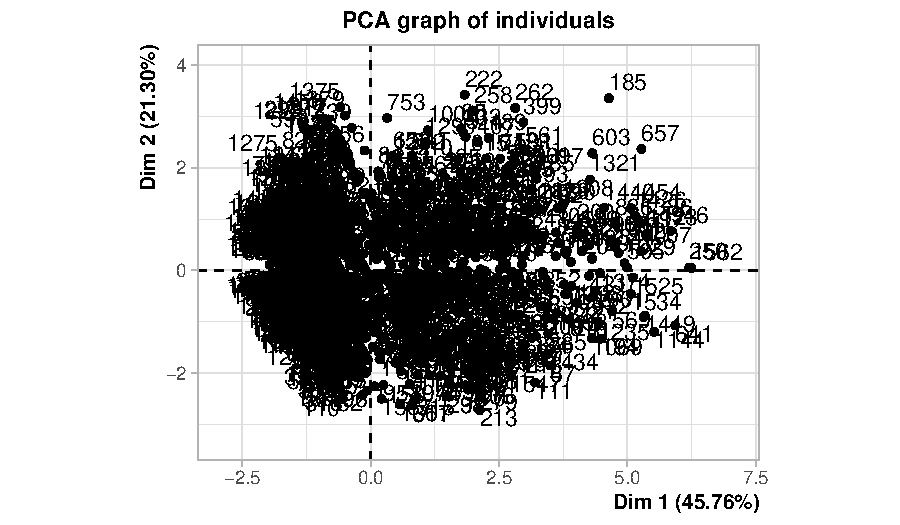
\includegraphics[width=\maxwidth]{figure/Analyse_factorielle-1} 

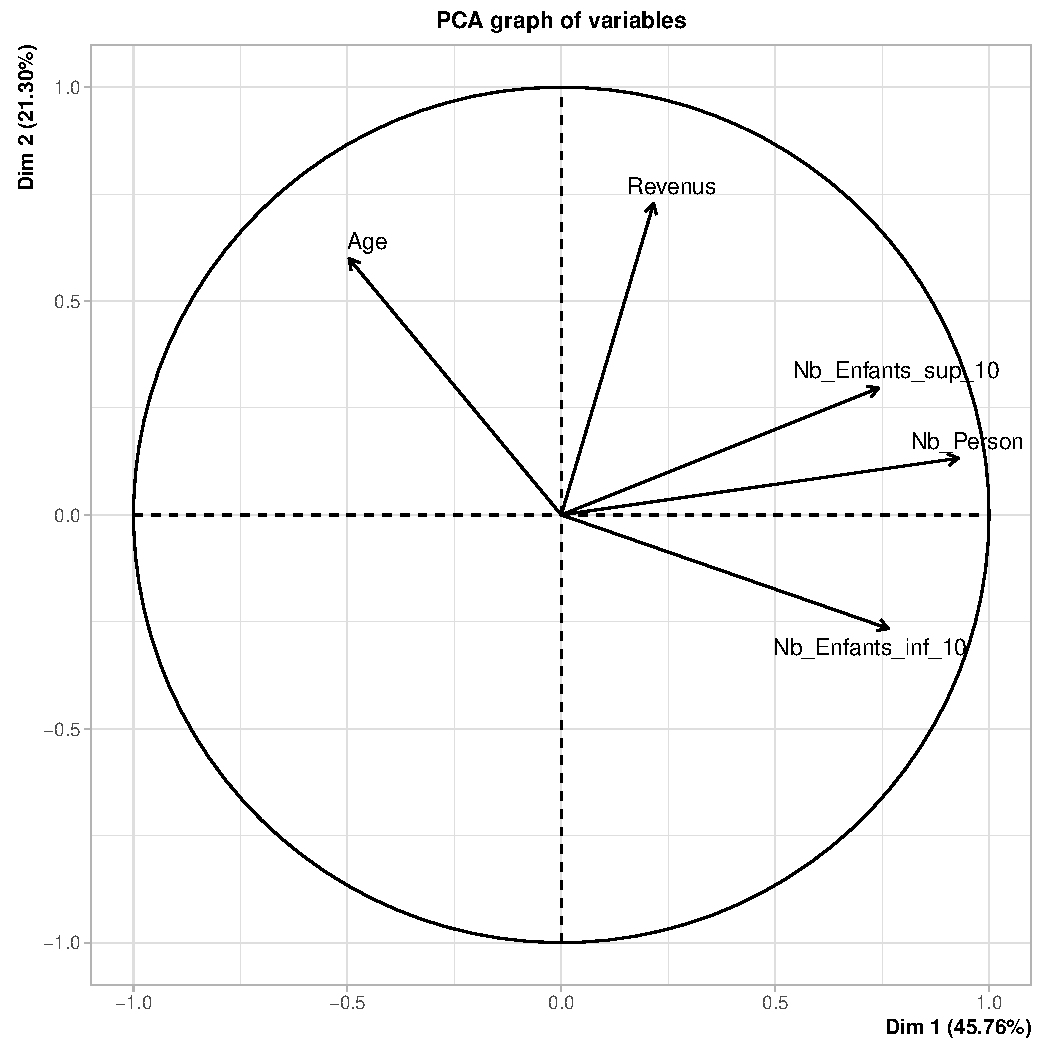
\includegraphics[width=\maxwidth]{figure/Analyse_factorielle-2} 
\begin{kframe}\begin{verbatim}
## 
## Call:
## PCA(X = quanti_meange) 
## 
## 
## Eigenvalues
##                        Dim.1   Dim.2   Dim.3   Dim.4   Dim.5
## Variance               2.288   1.065   0.892   0.586   0.169
## % of var.             45.756  21.302  17.842  11.729   3.371
## Cumulative % of var.  45.756  67.057  84.899  96.629 100.000
## 
## Individuals (the 10 first)
##                       Dist    Dim.1    ctr   cos2    Dim.2    ctr   cos2  
## 1                 |  1.595 | -0.674  0.013  0.178 | -1.318  0.104  0.683 |
## 2                 |  1.133 |  0.104  0.000  0.008 | -0.236  0.003  0.043 |
## 3                 |  1.897 | -0.899  0.023  0.225 | -1.447  0.125  0.582 |
## 4                 |  1.705 | -0.223  0.001  0.017 | -1.068  0.068  0.392 |
## 5                 |  2.842 |  1.562  0.068  0.302 | -0.240  0.003  0.007 |
## 6                 |  1.538 | -0.256  0.002  0.028 | -0.646  0.025  0.177 |
## 7                 |  1.968 |  0.599  0.010  0.093 | -1.797  0.194  0.834 |
## 8                 |  1.783 | -1.243  0.043  0.486 | -1.168  0.082  0.429 |
## 9                 |  2.719 | -0.631  0.011  0.054 | -2.250  0.303  0.685 |
## 10                |  2.462 |  0.998  0.028  0.164 | -1.033  0.064  0.176 |
##                    Dim.3    ctr   cos2  
## 1                  0.326  0.008  0.042 |
## 2                  0.153  0.002  0.018 |
## 3                 -0.251  0.004  0.017 |
## 4                 -0.851  0.052  0.249 |
## 5                 -1.730  0.214  0.371 |
## 6                  1.199  0.103  0.608 |
## 7                  0.028  0.000  0.000 |
## 8                  0.413  0.012  0.054 |
## 9                 -0.476  0.016  0.031 |
## 10                -0.218  0.003  0.008 |
## 
## Variables
##                      Dim.1    ctr   cos2    Dim.2    ctr   cos2    Dim.3    ctr
## Age               | -0.496 10.754  0.246 |  0.599 33.685  0.359 |  0.451 22.772
## Revenus           |  0.216  2.039  0.047 |  0.728 49.795  0.530 | -0.648 47.045
## Nb_Person         |  0.928 37.632  0.861 |  0.132  1.645  0.018 |  0.148  2.451
## Nb_Enfants_inf_10 |  0.764 25.540  0.584 | -0.265  6.617  0.070 | -0.161  2.892
## Nb_Enfants_sup_10 |  0.742 24.034  0.550 |  0.297  8.257  0.088 |  0.471 24.840
##                     cos2  
## Age                0.203 |
## Revenus            0.420 |
## Nb_Person          0.022 |
## Nb_Enfants_inf_10  0.026 |
## Nb_Enfants_sup_10  0.222 |
\end{verbatim}
\end{kframe}
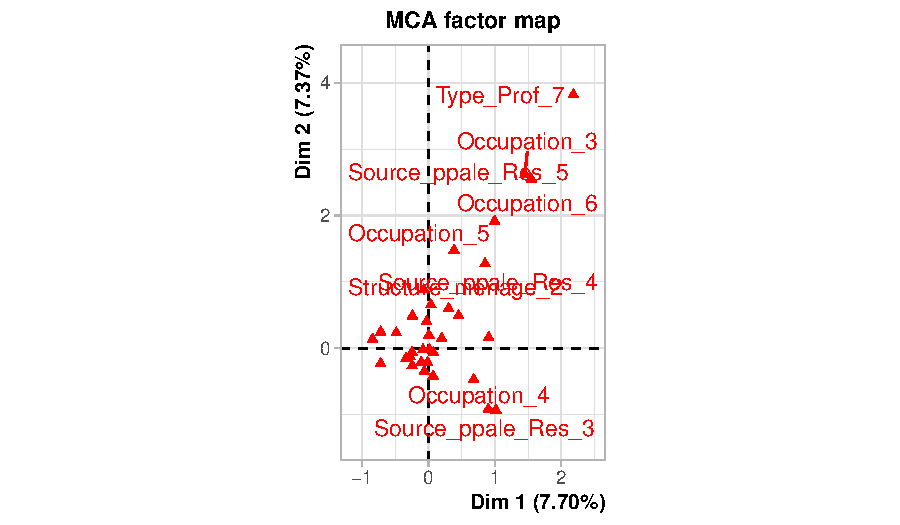
\includegraphics[width=\maxwidth]{figure/Analyse_factorielle-3} 

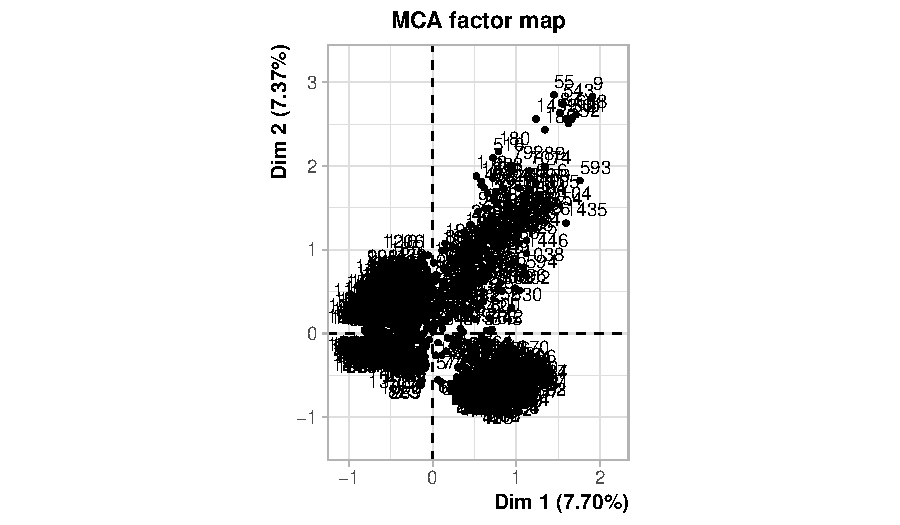
\includegraphics[width=\maxwidth]{figure/Analyse_factorielle-4} 
\begin{kframe}\begin{verbatim}
## 
## Call:
## MCA(X = quali_menage) 
## 
## 
## Eigenvalues
##                        Dim.1   Dim.2   Dim.3   Dim.4   Dim.5   Dim.6   Dim.7
## Variance               0.415   0.317   0.229   0.216   0.201   0.181   0.179
## % of var.              8.808   6.722   4.858   4.582   4.265   3.845   3.803
## Cumulative % of var.   8.808  15.530  20.388  24.970  29.235  33.080  36.882
##                        Dim.8   Dim.9  Dim.10  Dim.11  Dim.12  Dim.13  Dim.14
## Variance               0.170   0.168   0.156   0.155   0.148   0.147   0.143
## % of var.              3.597   3.564   3.307   3.279   3.132   3.120   3.028
## Cumulative % of var.  40.479  44.043  47.350  50.629  53.761  56.881  59.909
##                       Dim.15  Dim.16  Dim.17  Dim.18  Dim.19  Dim.20  Dim.21
## Variance               0.142   0.141   0.139   0.136   0.132   0.130   0.123
## % of var.              3.003   2.980   2.948   2.886   2.792   2.752   2.606
## Cumulative % of var.  62.912  65.892  68.840  71.727  74.518  77.270  79.877
##                       Dim.22  Dim.23  Dim.24  Dim.25  Dim.26  Dim.27  Dim.28
## Variance               0.119   0.115   0.108   0.105   0.101   0.097   0.084
## % of var.              2.532   2.439   2.301   2.232   2.151   2.060   1.785
## Cumulative % of var.  82.408  84.847  87.149  89.381  91.531  93.591  95.377
##                       Dim.29  Dim.30  Dim.31  Dim.32  Dim.33
## Variance               0.076   0.065   0.047   0.021   0.009
## % of var.              1.606   1.383   1.000   0.435   0.199
## Cumulative % of var.  96.983  98.366  99.366  99.801 100.000
## 
## Individuals (the 10 first)
##                  Dim.1    ctr   cos2    Dim.2    ctr   cos2    Dim.3    ctr
## 1             |  0.526  0.043  0.087 | -0.298  0.018  0.028 |  0.167  0.008
## 2             |  0.649  0.065  0.066 |  0.361  0.026  0.020 | -1.173  0.384
## 3             |  0.331  0.017  0.028 |  0.516  0.054  0.068 | -0.085  0.002
## 4             |  0.497  0.038  0.073 | -0.384  0.030  0.044 |  0.099  0.003
## 5             |  0.556  0.048  0.062 |  0.019  0.000  0.000 | -0.560  0.088
## 6             |  0.621  0.059  0.063 |  0.519  0.054  0.044 | -1.705  0.810
## 7             |  0.550  0.046  0.139 | -0.440  0.039  0.089 |  0.014  0.000
## 8             |  0.323  0.016  0.027 |  0.401  0.032  0.041 |  0.176  0.009
## 9             |  0.145  0.003  0.001 |  3.177  2.032  0.490 |  1.343  0.502
## 10            |  0.403  0.025  0.006 |  1.096  0.242  0.047 | -1.353  0.510
##                 cos2  
## 1              0.009 |
## 2              0.216 |
## 3              0.002 |
## 4              0.003 |
## 5              0.063 |
## 6              0.472 |
## 7              0.000 |
## 8              0.008 |
## 9              0.087 |
## 10             0.072 |
## 
## Categories (the 10 first)
##                   Dim.1     ctr    cos2  v.test     Dim.2     ctr    cos2
## Sexe_1        |  -0.073   0.065   0.003  -2.129 |   0.685   7.401   0.253
## Sexe_2        |   0.040   0.035   0.003   2.129 |  -0.369   3.991   0.253
## Diplome_Max_1 |   0.071   0.019   0.001   0.987 |   0.129   0.082   0.002
## Diplome_Max_2 |  -0.090   0.010   0.000  -0.689 |   0.013   0.000   0.000
## Diplome_Max_3 |   0.353   0.319   0.010   3.963 |   0.239   0.192   0.005
## Diplome_Max_4 |  -0.018   0.003   0.000  -0.456 |  -0.025   0.008   0.000
## Diplome_Max_5 |   0.058   0.010   0.000   0.707 |  -0.228   0.205   0.005
## Diplome_Max_6 |  -0.659   1.498   0.048  -8.706 |   0.086   0.033   0.001
## Diplome_Max_7 |   0.448   0.581   0.018   5.372 |  -0.130   0.064   0.002
## Diplome_Max_8 |  -0.026   0.003   0.000  -0.366 |   0.198   0.197   0.005
##                v.test     Dim.3     ctr    cos2  v.test  
## Sexe_1         19.893 |  -0.646   9.107   0.225 -18.760 |
## Sexe_2        -19.893 |   0.348   4.911   0.225  18.760 |
## Diplome_Max_1   1.791 |  -0.228   0.353   0.006  -3.155 |
## Diplome_Max_2   0.099 |  -0.690   1.060   0.018  -5.254 |
## Diplome_Max_3   2.683 |  -0.197   0.181   0.003  -2.214 |
## Diplome_Max_4  -0.624 |  -0.164   0.487   0.011  -4.149 |
## Diplome_Max_5  -2.794 |  -0.223   0.271   0.005  -2.730 |
## Diplome_Max_6   1.135 |   0.100   0.063   0.001   1.326 |
## Diplome_Max_7  -1.562 |   0.619   2.014   0.035   7.431 |
## Diplome_Max_8   2.774 |   0.065   0.030   0.001   0.916 |
## 
## Categorical variables (eta2)
##                    Dim.1 Dim.2 Dim.3  
## Sexe             | 0.003 0.253 0.225 |
## Diplome_Max      | 0.071 0.023 0.107 |
## Type_Prof        | 0.015 0.257 0.300 |
## Occupation       | 0.865 0.545 0.262 |
## Source_ppale_Res | 0.928 0.484 0.144 |
## Structure_menage | 0.115 0.330 0.235 |
## TYPEMEN          | 0.908 0.326 0.330 |
\end{verbatim}


{\ttfamily\noindent\bfseries\color{errorcolor}{\#\# Error in MFA(data\_menage, group = c(5, 6), type = c(rep("{}s"{}, 1), rep("{}n"{}, : not convenient group definition}}\end{kframe}
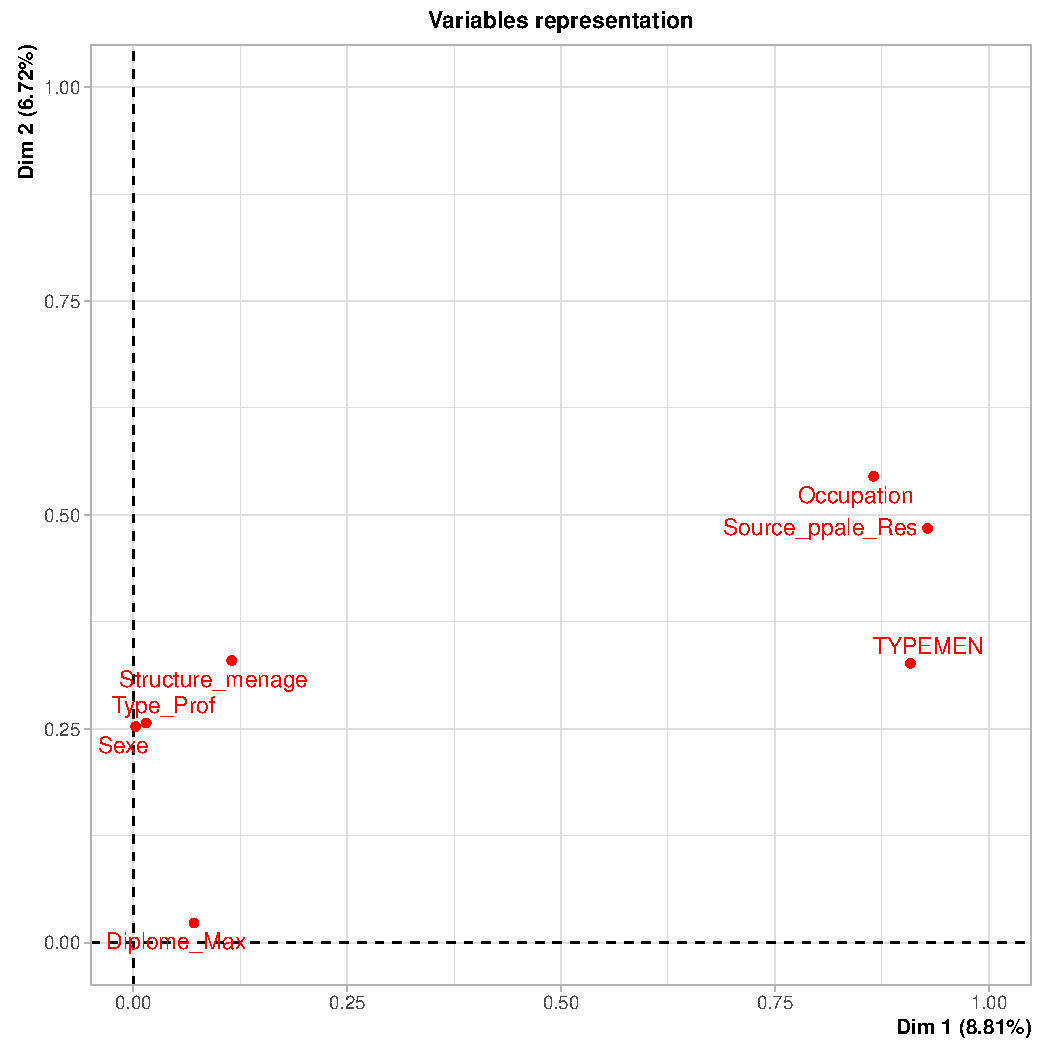
\includegraphics[width=\maxwidth]{figure/Analyse_factorielle-5} 
\end{knitrout}




%-------------------------------------------------------------------------------
%  SECTION 1: Variables quantitatives
%-------------------------------------------------------------------------------
\subsection{Analyse descriptive des variables quantitatives }
\subsubsection{Analyse univarié}

\begin{table*}[!h] \centering
%\ra{1.3}
\begin{small}
\begin{tabular}{@{}lrrrrrr@{}}\toprule
\textbf{Variables}& \textbf{Moyenne} & \textbf{Médiane}& \textbf{Min} & \textbf{Maximum} & \textbf{Variance} & \textbf{Ecart-type} \\ \midrule
\textbf{Age}          & 51.87 &  52 & 18 & 89 & 209.91 & 14.49\ \\ \hdashline
\textbf{Revenus}      & 2~573.20 & 2~349 & 535&7~600 & 1~967~644.23&1~402.73   \\ \hdashline
\textbf{Nombre d'enfants dont âge > 10 ans} &  0.44 & 0 & 0 & 3 & 0.67 & 0.82  \\  \hdashline
\textbf{Nombre d'enfants dont âge <= 10 ans} &  0.32 & 0 & 0 & 3 & 0.48 & 0.70 \\  
\bottomrule
\end{tabular}
\end{small}
\caption{Statistiques descriptives des variables quantitatives}
\end{table*}


%-------------------------------------------------------------------------------
%   SECTION 2: Variables qualitatives
%-------------------------------------------------------------------------------

\end{document}

